\begin{enumerate}
	\item L'administrateur se connecte au site avec ses identifiant. 
	\item Un nouveau bouton de navigation apparait dans la bar de navigation. 
	\item L'administrateur clique sur le bouton \textit{Admin}
	\item Il sélectionne \textit{Type Session} dans le menu déroulant. 
	\item L'administrateur atterris sur la page de gestion des type de sessions. 
	\item Il clique sur le bouton edit
	\item Un formulaire apparait et il le remplis avec les bonne information (jour - heure [hh:mm])
	\item Il clique sur \textit{ok} 
\end{enumerate}

\vspace{\baselineskip}
\begin{figure}[h]
	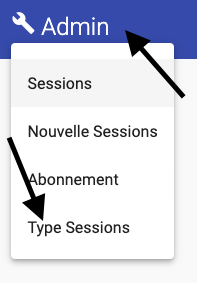
\includegraphics[width=0.4\textwidth,center]{Figures/us13-1}
	\caption{Menu de l'administrateur}
\end{figure}

\newpage
\begin{figure}[h]
	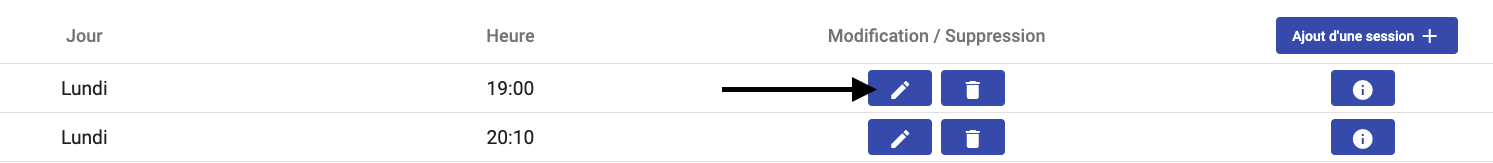
\includegraphics[width=0.9\textwidth,center]{Figures/us13-2}
	\caption{Bouton de modification du type de session}
\end{figure}

\vspace{\baselineskip}
\begin{figure}[h]
	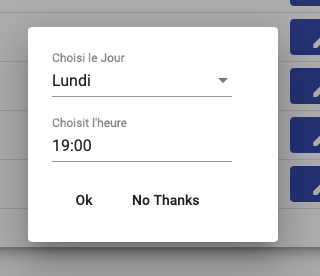
\includegraphics[width=0.4\textwidth,center]{Figures/us13-3}
	\caption{Formulaire de modification du type de session}
\end{figure}

\subsubsection{Gestion des erreurs}
	\paragraph{}
		Chaque type de sessions est unique, si l'administrateur rentre des informations correspondant à un type de sessions deja existant, une erreur apparaitra au dessus du formulaire.